% Modelo SBrT adaptado para o trabalho do grupo
\documentclass[english,hidelinks]{sbrt}
\usepackage[brazil]{babel}
\usepackage[utf8]{inputenc}
\usepackage{graphicx}
\usepackage{subfigure}
\usepackage{amsmath}
\usepackage{url}
\usepackage{cite}
\usepackage{float}
\usepackage{hyperref}
\usepackage{caption}
\captionsetup{
  font=footnotesize,
  labelsep=period,
  format=plain,
  justification=raggedright,
  singlelinecheck=false
}

% Título e autores
\begin{document}
\title{Sistema de Monitoramento de Papel em Dispensers Utilizando Sensor Ultrassônico e Protocolo MQTT}
\author{Arthur Peixoto Schiller, Franc Wang e Juliana de Oliveira\\IBMEC - Sistemas Embarcados e IoT}
\maketitle

\markboth{XLIII SIMPÓSIO BRASILEIRO DE TELECOMUNICAÇÕES E PROCESSAMENTO DE SINAIS - SBrT 2025, 29 DE SETEMBRO A 2 DE OUTUBRO, NATAL, RN}{}

\begin{abstract}
Este trabalho apresenta o desenvolvimento de um sistema protótipo para monitoramento em tempo real do nível de papel em dispensers, utilizando sensor ultrassônico e comunicação via protocolo MQTT. O principal objetivo é reduzir a insatisfação dos usuários causada pela falta de reposição, especialmente em locais com alto fluxo de pessoas. O sensor detecta o nível de papel e envia alertas automaticamente ao responsável pela manutenção sempre que valores críticos são atingidos. O sistema proposto é de baixo custo, fácil replicação e alta escalabilidade. A visualização das informações ocorre por meio de um aplicativo mobile desenvolvido com React Native.
\end{abstract}
\begin{keywords}
Monitoramento, Dispenser, Sensor Ultrassônico, MQTT, IoT.
\end{keywords}

\section{Introdução}
Vivemos atualmente na \textbf{Era da Experiência}, em que empresas precisam oferecer experiências únicas aos clientes, indo além da simples entrega de produtos ou serviços. Fatores como limpeza, organização e disponibilidade de itens essenciais influenciam diretamente a percepção de qualidade e conforto, impactando o tempo de permanência do cliente e sua disposição para retornar. A experiência do usuário tornou-se um pilar fundamental para o sucesso de qualquer negócio. Diante disso, propõe-se um sistema para monitorar o nível de papel em dispensers utilizando sensor ultrassônico e comunicação MQTT. Ao detectar que o papel está acabando, o sistema emite um alerta, permitindo a reposição antes que o papel se esgote totalmente.

\section{Descrição do Sistema}
O sistema é composto por:
\begin{itemize}
    \item Sensor ultrassônico HC-SR04 (alcance de até 4 metros);
    \item Microcontrolador ESP32 CP2103;
    \item Comunicação via protocolo MQTT utilizando o broker Mosquitto;
    \item Aplicativo mobile desenvolvido em React Native com Expo e JavaScript;
    \item Biblioteca Paho-MQTT para integração com o MQTT;
    \item Alimentação por bateria (em testes);
    \item Frequência de envio: 200 ms.
\end{itemize}
O sensor de distância é posicionado no topo do dispenser, medindo a distância até o topo da pilha de papéis. Quando o reservatório está cheio, essa distância é mínima; à medida que os papéis são retirados, a distância aumenta. Ao atingir 70\% da altura total, o sistema interpreta como limite crítico e emite alerta de reposição. A comunicação é realizada via MQTT, segmentada em três tópicos: porcentagem atual de papel, status descritivo ("cheio", "precisa repor" ou "vazio") e valor da distância em centímetros. Notificações são enviadas apenas em condição crítica, otimizando o tráfego de dados.

\begin{figure}[H]
  \centering
  \fbox{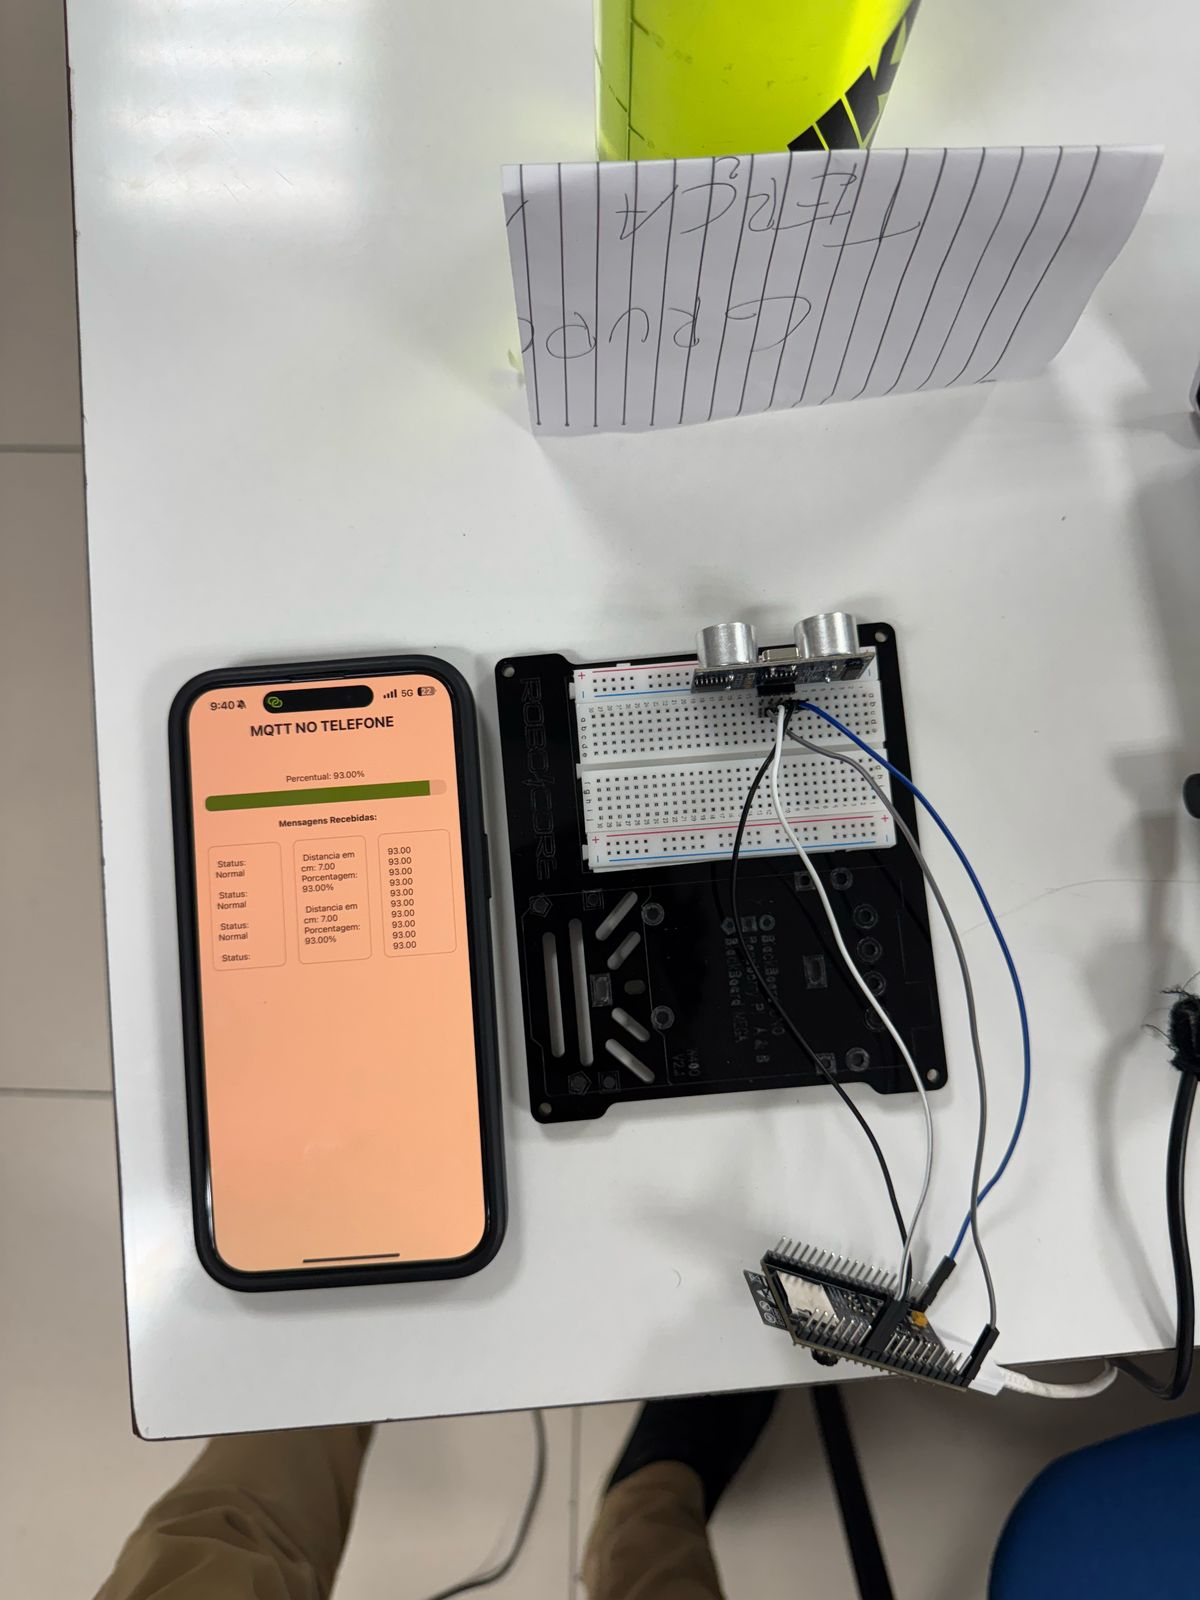
\includegraphics[width=0.4\textwidth]{montagemSistema.jpg}}
  \caption{Protótipo do sistema instalado com sensor ultrassônico e ESP montado em bancada.}
  \label{fig:sistema}
\end{figure}

\section{Testes e Validação}
Foram realizados três testes em bancada, conduzidos em ambiente laboratorial. Os resultados indicaram acurácia moderada nas medições, suficiente para validar a viabilidade funcional do sistema. Como parte da arquitetura de monitoramento remoto, foi desenvolvido um aplicativo mobile com React Native que se comunica com o sistema embarcado via MQTT, permitindo visualização em tempo real do estado dos dispensadores. A interface web simplifica o acompanhamento e a tomada de decisão.

Direcionamento técnico para etapas futuras:
\begin{itemize}
    \item Melhorias no layout da interface web, com foco em responsividade;
    \item Dashboard administrativo para múltiplos dispositivos;
    \item Implementação de alertas visuais e sonoros para eventos críticos.
\end{itemize}

\begin{figure}[H]
  \centering
  \fbox{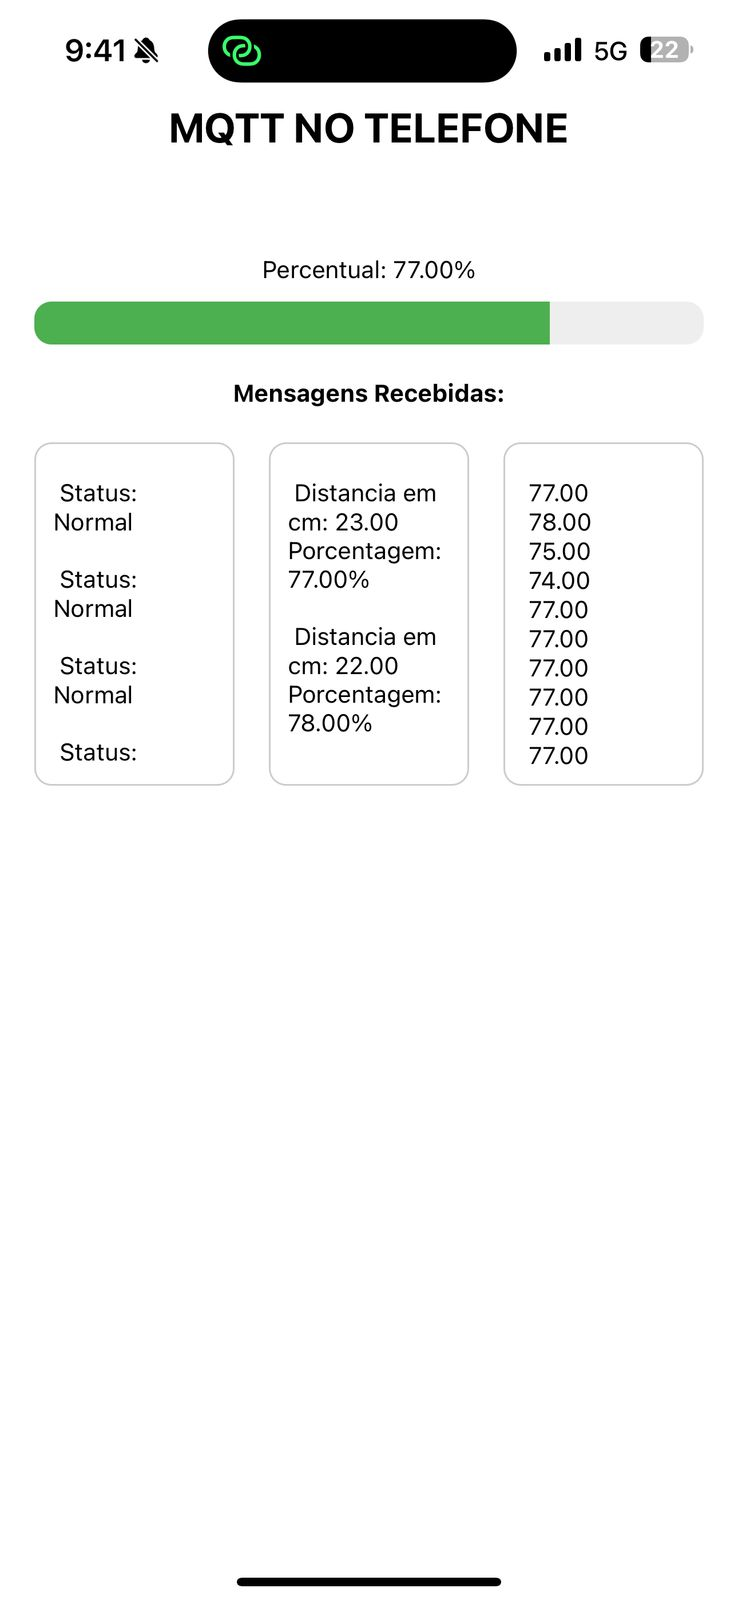
\includegraphics[width=0.3\textwidth]{printApp.jpg}}
  \caption{Tela principal do app desenvolvido para acompanhamento dos dados via MQTT.}
  \label{fig:app}
\end{figure}

\section{Resultados Experimentais e Desempenho Quantitativo}
Para avaliar a precisão e repetibilidade do sistema, foram realizados cinco experimentos com o sensor ultrassônico, variando a distância do papel ao sensor (2, 7, 12, 17 e 22 cm). Cada teste gerou um conjunto de 500 amostras, analisadas quantitativamente conforme descrito a seguir.

% Gráficos menores para caber em até 3 páginas

% Boxplot das Distâncias
\begin{figure}[H]
    \centering
    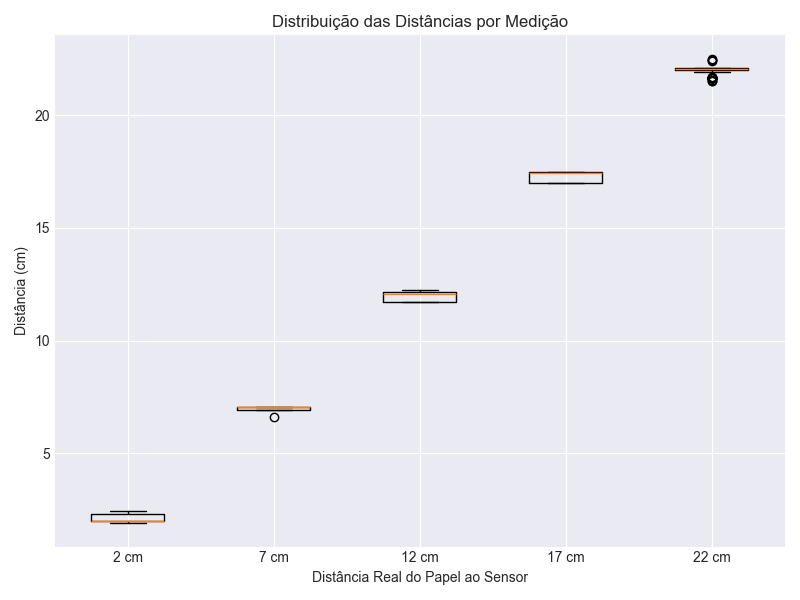
\includegraphics[width=0.28\textwidth]{graficos/boxplot_distancias.png}
    \caption{Boxplot das leituras do sensor para diferentes distâncias do papel ao sensor.}
    \label{fig:boxplot_distancias}
\end{figure}

% Desvio Padrão das Medições
\begin{figure}[H]
    \centering
    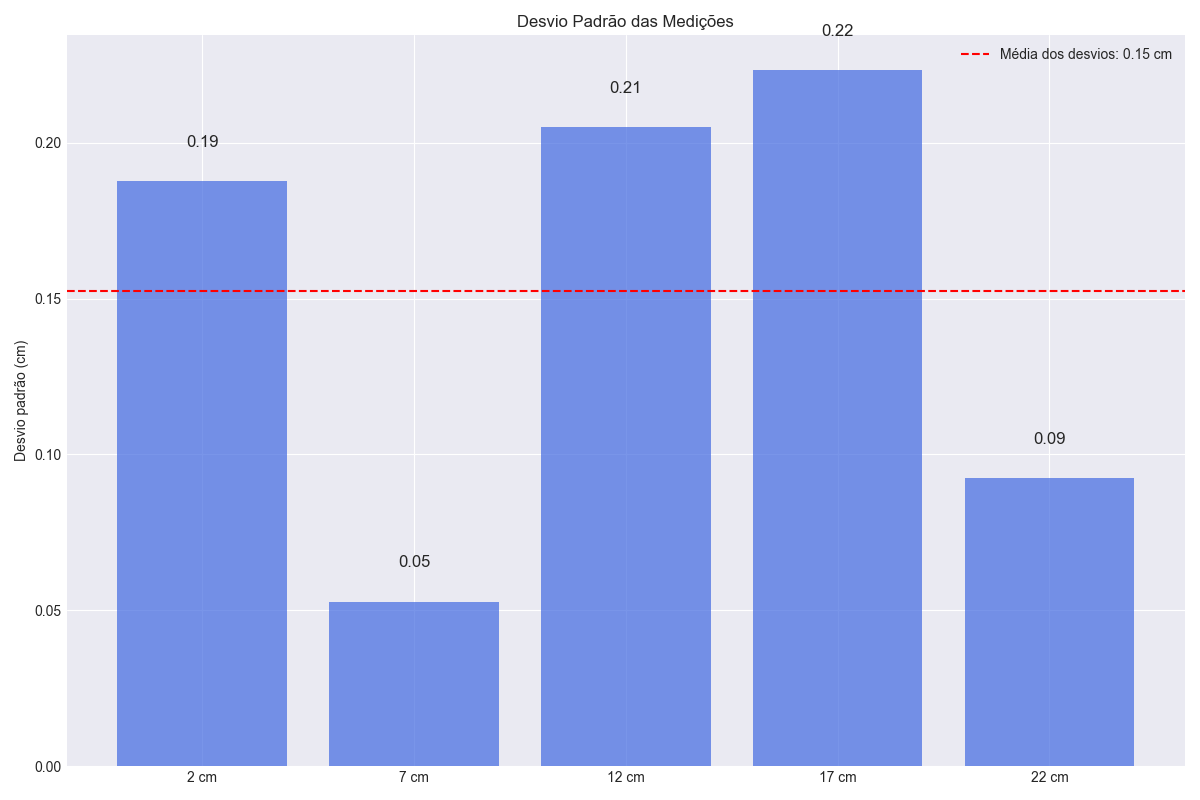
\includegraphics[width=0.28\textwidth]{graficos/desvios_padrao.png}
    \caption{Desvio padrão das leituras do sensor para cada posição do papel.}
    \label{fig:desvios_padrao}
\end{figure}

% Evolução Temporal das Leituras
\begin{figure}[H]
    \centering
    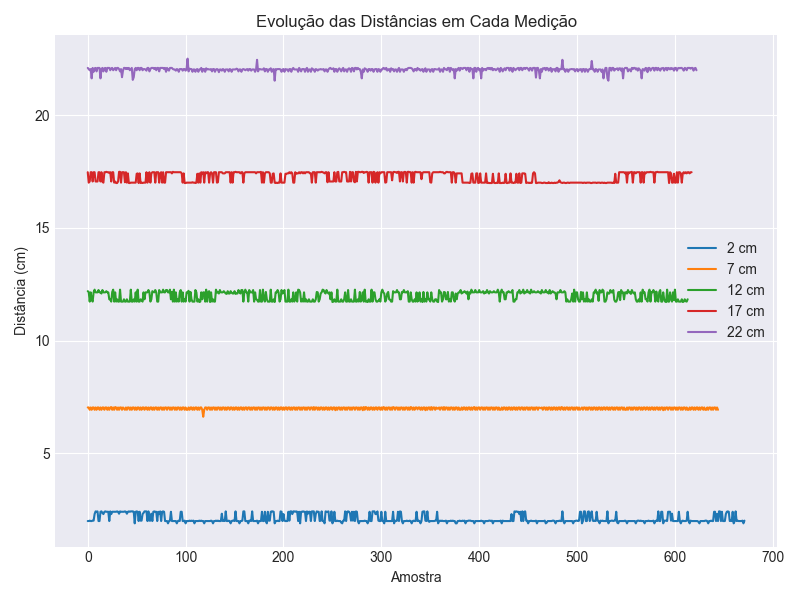
\includegraphics[width=0.28\textwidth]{graficos/series_temporais.png}
    \caption{Evolução temporal das leituras do sensor para diferentes distâncias.}
    \label{fig:series_temporais}
\end{figure}

% Amplitude das Medições
\begin{figure}[H]
    \centering
    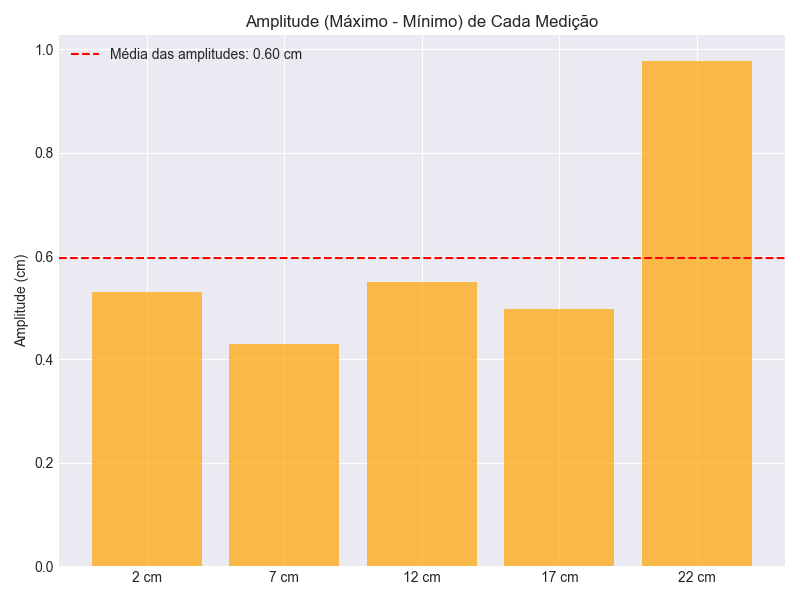
\includegraphics[width=0.28\textwidth]{graficos/amplitudes.png}
    \caption{Amplitude das leituras do sensor para cada posição do papel.}
    \label{fig:amplitudes}
\end{figure}

\subsection{Taxa de Erro Percentual}
A precisão global do sistema foi avaliada pelo erro percentual médio (MAPE), comparando a média das leituras com a distância real. A Figura~\ref{fig:erro_percentual} apresenta o erro percentual de cada teste e o MAPE global (linha vermelha), que se manteve baixo em todas as condições, indicando excelente desempenho para aplicações de monitoramento de estoque.

\begin{figure}[H]
    \centering
    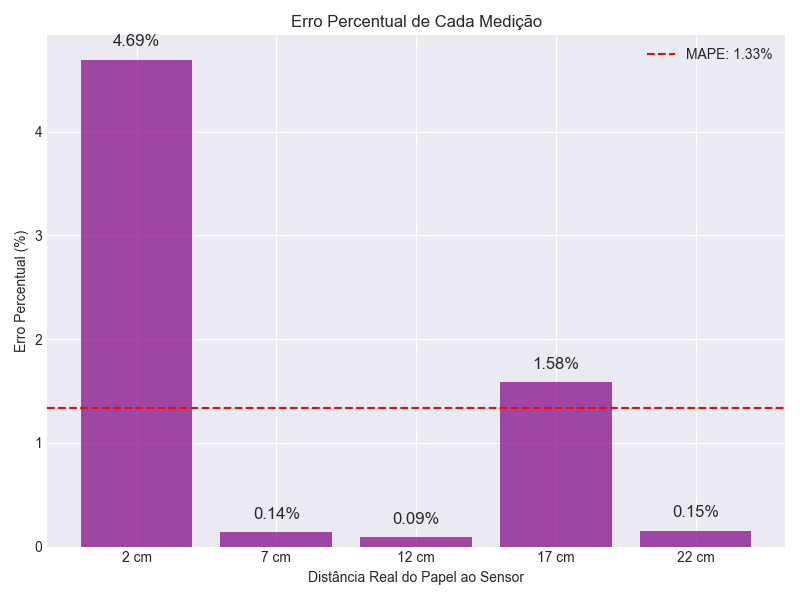
\includegraphics[width=0.45\textwidth]{graficos/erro_percentual.png}
    \caption{Erro percentual médio das medições do sistema em relação às distâncias reais.}
    \label{fig:erro_percentual}
\end{figure}

Esses resultados demonstram que o sistema apresenta alta precisão, baixa variabilidade e excelente confiabilidade para o monitoramento do nível de papel em dispensers, sendo adequado para aplicações reais de IoT e controle de estoque.

\section{Conclusão}
Os resultados experimentais demonstraram que o sistema desenvolvido apresenta alta precisão e confiabilidade para o monitoramento do nível de papel em dispensers. O erro percentual médio (MAPE) obtido nos testes foi baixo, e o erro médio absoluto ficou em torno de poucos milímetros a 1 cm, mesmo nas diferentes faixas de operação do sensor. Considerando que o controle de estoque de papel não exige precisão milimétrica, esse erro é absolutamente irrisório para a aplicação proposta. Na prática, pequenas variações não impactam a reposição eficiente do papel, garantindo que alertas sejam emitidos de forma confiável e sem alarmes falsos. Portanto, o sistema atende plenamente aos requisitos de um monitoramento automatizado, sendo robusto, de baixo custo e facilmente replicável para ambientes reais. O uso de sensores ultrassônicos, aliado à análise quantitativa dos dados, mostrou-se uma solução eficaz para aplicações de IoT voltadas ao controle de insumos em tempo real.

% Adendo sobre limitações do sensor
\textbf{Nota:} O sensor ultrassônico utilizado apresenta baixa precisão para distâncias menores que 2 cm. Por isso, nos experimentos, o recipiente de 20 cm foi testado com o papel posicionado a pelo menos 2 cm do sensor, evitando a faixa de menor performance e garantindo maior confiabilidade nas medições.

\bibliographystyle{IEEEtran}
% \bibliography{refs} % Se houver referências, descomente e ajuste

\end{document}
